\documentclass{report}
\usepackage[english]{babel}
\usepackage[utf8x]{inputenc}
\usepackage{amsmath}
\usepackage{multicol}
\usepackage{multirow}
\usepackage{listings}
\usepackage{tikz}

% TODO:
% - set lstlistings font

\begin{document}

\section{Header}

All GENPRO-1 files begin with a 6-bit text header using a custom encoding which
is broken into two parts. The header contains no newline characters. Each line
in the header (in both parts) is 100 characters long. The first part of the
header is 11 lines long and contains:
\begin{itemize}
	\item The number of parameters contained in the file.
	\item The scale and offset (``bias") for each parameter (field).
	\item The cycle rate; i.e., how much time is elapsed between each batch of
	      samples.
\end{itemize}

There are no

%Format strings for parsing the header:
%
%\begin{lstlisting}
%format (10(1x,14a8,/))
%format (1x,i2,26x,i4,70x,i3)
%format (/," item   location   rate",17x,"description",20x,"name",4x,"units"18x,"scale",12x,"bias",/)
%format (4x,i3,1x,i4,5x,7a8,10x,f7.1,3x,f7.1)
%format (i3,1x,i4,5x,7a8,10x,f7.1,3xf7.1)
%\end{lstlisting}

%files appear to contain some number of records, each record 

% This one is just used for printing header info
% format ((1x,i3,*)*,i8,i9,5x,7a8,17x,f9.2,5x,f9.2)

\subsection{6-bit Character Encoding}

\begin{table}
\centering
\caption{GenPro Character Encoding}
\label{Tbl.}
\begin{tabular}{|rrr|rrrl|}
\multicolumn{3}{c}{GENPRO-1} & \multicolumn{4}{c}{ASCII} \\
\hline
Dec & Hex & Oct & Hex & Dec & Oct & Character \\
\hline
% Dec       Hex       Oct       Dec       Hex       Oct
\(  0\) & \(  0\) & \(  0\) & \( 58\) & \( 3\mathtt{A}\) & \( 72\) & \texttt{:} \\
\hline
\(1\)--\(26\) & % Genpro Dec
\(1\)--\(1\mathtt{A}\) & % Genpro Hex
\(1\)--\(32\) & % Genpro Oct
\( 66\) & % ASCII Dec
\( 42\) & % ASCII Hex
\(102\) & % ASCII Oct
\texttt{A}--\texttt{Z} \\ % ASCII Char
\hline
\(27\)--\(36\) & % Genpro Dec
\(1\mathtt{B}\)--\(24\) & % Genpro Hex
\(33\)--\(44\) & % Genpro Oct
\( 48\) & % ASCII Dec
\( 30\) & % ASCII Hex
\( 60\) & % ASCII Oct
\texttt{0}--\texttt{9} \\ % ASCII Char
\hline
% Dec       Hex       Oct       Dec       Hex       Oct
\( 37\) & \( 25\) & \( 45\) & \( 43\) & \( 2\mathtt{B}\) & \( 53\) & \texttt{+} \\ \hline
\( 38\) & \( 26\) & \( 46\) & \( 45\) & \( 2\mathtt{D}\) & \( 55\) & \texttt{-} \\ \hline
\( 39\) & \( 27\) & \( 47\) & \( 42\) & \( 2\mathtt{A}\) & \( 52\) & \texttt{*} \\ \hline
\( 40\) & \( 28\) & \( 50\) & \( 47\) & \( 2\mathtt{F}\) & \( 57\) & \texttt{/} \\ \hline
\( 41\) & \( 29\) & \( 51\) & \( 40\) & \( 28\) & \( 50\) & \texttt{(} \\ \hline
\( 42\) & \( 2\mathtt{A}\) & \( 52\) & \( 41\) & \( 29\) & \( 51\) & \texttt{)} \\ \hline
\( 43\) & \( 2\mathtt{B}\) & \( 53\) & \( 36\) & \( 24\) & \( 44\) & \texttt{\$} \\ \hline
\( 44\) & \( 2\mathtt{C}\) & \( 54\) & \( 61\) & \( 3\mathtt{D}\) & \( 75\) & \texttt{=} \\ \hline
\( 45\) & \( 2\mathtt{D}\) & \( 55\) & \( 32\) & \( 20\) & \( 40\) & Space \\ \hline
\( 46\) & \( 2\mathtt{E}\) & \( 56\) & \( 44\) & \( 2\mathtt{C}\) & \( 54\) & \texttt{,} \\ \hline
\( 47\) & \( 2\mathtt{F}\) & \( 57\) & \( 46\) & \( 2\mathtt{E}\) & \( 56\) & \texttt{.} \\ \hline
\( 48\) & \( 30\) & \( 60\) & \( 35\) & \( 23\) & \( 43\) & \texttt{\#} \\ \hline
\( 49\) & \( 31\) & \( 61\) & \( 91\) & \( 5\mathtt{B}\) & \(133\) & \texttt{[} \\ \hline
\( 50\) & \( 32\) & \( 62\) & \( 93\) & \( 5\mathtt{D}\) & \(135\) & \texttt{]} \\ \hline
\( 51\) & \( 33\) & \( 63\) & \( 37\) & \( 25\) & \( 45\) & \texttt{\%} \\ \hline
\( 52\) & \( 34\) & \( 64\) & \( 34\) & \( 22\) & \( 42\) & \texttt{"} \\ \hline
\( 53\) & \( 35\) & \( 65\) & \( 95\) & \( 5\mathtt{F}\) & \(137\) & \texttt{\_} \\ \hline
\( 54\) & \( 36\) & \( 66\) & \( 33\) & \( 21\) & \( 41\) & \texttt{!} \\ \hline
\( 55\) & \( 37\) & \( 67\) & \( 38\) & \( 26\) & \( 46\) & \texttt{\&} \\ \hline
\( 56\) & \( 38\) & \( 70\) & \( 39\) & \( 27\) & \( 47\) & \texttt{'} \\ \hline
\( 57\) & \( 39\) & \( 71\) & \( 63\) & \( 3\mathtt{F}\) & \( 77\) & \texttt{?} \\ \hline
\( 58\) & \( 3\mathtt{A}\) & \( 72\) & \( 60\) & \( 3\mathtt{C}\) & \( 74\) & \texttt{<} \\ \hline
\( 59\) & \( 3\mathtt{B}\) & \( 73\) & \( 62\) & \( 3\mathtt{E}\) & \( 76\) & \texttt{>} \\ \hline
\( 60\) & \( 3\mathtt{C}\) & \( 74\) & \( 64\) & \( 40\) & \(100\) & \texttt{@} \\ \hline
\( 61\) & \( 3\mathtt{D}\) & \( 75\) & \( 92\) & \( 5\mathtt{C}\) & \(134\) & \texttt{\textbackslash} \\ \hline
\( 62\) & \( 3\mathtt{E}\) & \( 76\) & \( 94\) & \( 5\mathtt{E}\) & \(136\) & \texttt{\^} \\ \hline
\( 63\) & \( 3\mathtt{F}\) & \( 77\) & \( 59\) & \( 3\mathtt{B}\) & \( 73\) & \texttt{;} \\ \hline
\end{tabular}
\end{table}

\section{Data section}

The offset, in multiples of 8-bit bytes, from the start of the file to the data section is computed as
\[
	8 \left \lceil \dfrac{100\times(11+N)\times6}{64} \right \rceil \mathrm{,}
\]

\noindent where \(N\) is the number of parameters in the file; i.e., the offset is in multiples of 64-bit words (owing to the Cray-1's 64-bit word size). For example, for the PHOENIX-78 dataset, \(N = 67\), so
\[
	8 \left \lceil \dfrac{100\times(11+67)\times 6}{64} \right \rceil = 5856 \mathrm{.}
\]

The stride between successive sets of sample data, in multiples of 8-bit bytes, is
\[
	8 \left \lceil \dfrac{M}{64} \right \rceil \mathrm{,}
\]

\noindent where \(M\) is the number of samples per cycle, as indicated in the header; \(M\) is given by
\[
	M = \sum_{i=0}^{N} R_i \mathrm{,}
\]

\noindent where \(N\) is again the number of parameters, and \(R_i\) is the sample rate for the \(i\)th parameter.

\begin{figure}
	\centering
	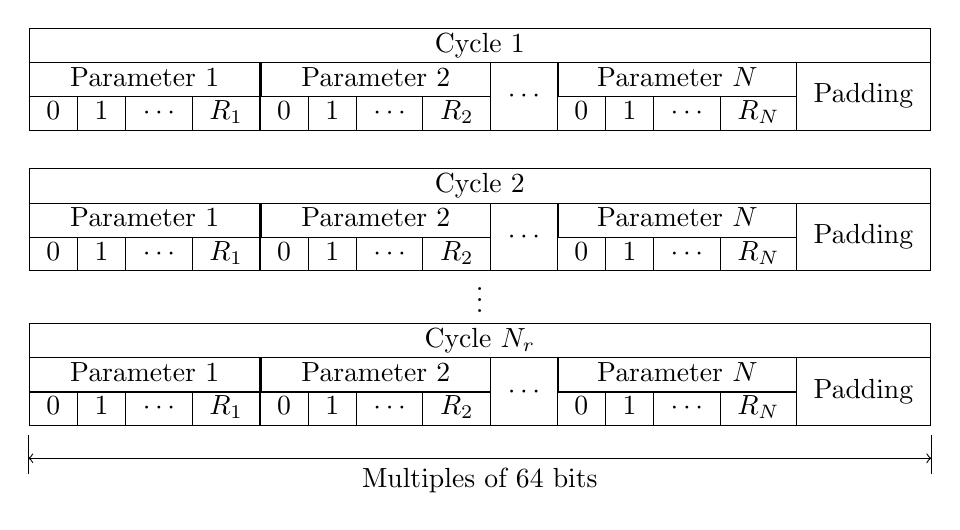
\begin{tikzpicture}
	\node (table) [inner sep=0pt] {
		\begin{tabular}{@{}|c|c|c|c|c|c|c|c|c|c|c|c|c|c|@{}}
			\hline
				\multicolumn{14}{|c|}{Cycle \(1\)} \\
			\hline
				\multicolumn{4}{|c|}{Parameter \(1\)} &
				\multicolumn{4}{|c|}{Parameter \(2\)} &
				\multirow{2}{*}{\(\cdots\)} &
				\multicolumn{4}{|c|}{Parameter \(N\)} &
				\multirow{2}{*}{Padding} \\
			\cline{1-8}
			\cline{10-13}
				0 & 1 & \(\cdots\) & \(R_1\) &
				0 & 1 & \(\cdots\) & \(R_2\) & &
				0 & 1 & \(\cdots\) & \(R_N\) & \\
			\hline
			\multicolumn{8}{c}{\raisebox{1em}{}} \\
			\hline
				\multicolumn{14}{|c|}{Cycle \(2\)} \\
			\hline
				\multicolumn{4}{|c|}{Parameter \(1\)} &
				\multicolumn{4}{|c|}{Parameter \(2\)} &
				\multirow{2}{*}{\(\cdots\)} &
				\multicolumn{4}{|c|}{Parameter \(N\)} &
				\multirow{2}{*}{Padding} \\
			\cline{1-8}
			\cline{10-13}
				0 & 1 & \(\cdots\) & \(R_1\) &
				0 & 1 & \(\cdots\) & \(R_2\) & &
				0 & 1 & \(\cdots\) & \(R_N\) & \\
			\hline
			\multicolumn{14}{c}{\(\vdots\)} \\
			\hline
				\multicolumn{14}{|c|}{Cycle \(N_r\)} \\
			\hline
				\multicolumn{4}{|c|}{Parameter \(1\)} &
				\multicolumn{4}{|c|}{Parameter \(2\)} &
				\multirow{2}{*}{\(\cdots\)} &
				\multicolumn{4}{|c|}{Parameter \(N\)} &
				\multirow{2}{*}{Padding} \\
			\cline{1-8}
			\cline{10-13}
				0 & 1 & \(\cdots\) & \(R_1\) &
				0 & 1 & \(\cdots\) & \(R_2\) & &
				0 & 1 & \(\cdots\) & \(R_N\) & \\
			\hline
		\end{tabular}};
		\foreach \i/\corner in {1/south west, 2/south east}
			\draw (table.\corner) ++(down:3pt) -- ++(down:0.3cm)
			      coordinate (p\i) -- ++(down:0.2cm);
		\draw [<->] (p1) -- (p2)
		      node [midway,anchor=north] {Multiples of 64 bits};
	\end{tikzpicture}
	\caption{Data organization.}
	\label{Fig.DataOrganization}
\end{figure}

\end{document}
